% Copyright 2004 by Till Tantau <tantau@users.sourceforge.net>.
%
% In principle, this file can be redistributed and/or modified under
% the terms of the GNU Public License, version 2.
%
% However, this file is supposed to be a template to be modified
% for your own needs. For this reason, if you use this file as a
% template and not specifically distribute it as part of a another
% package/program, I grant the extra permission to freely copy and
% modify this file as you see fit and even to delete this copyright
% notice.

\documentclass[11pt]{beamer}
\usepackage{subcaption}
\usepackage{arydshln}
\usepackage{amsthm}
\usepackage{booktabs}
\usepackage{xcolor}
\usepackage{multirow}
\usepackage{caption}
\usepackage{kotex}
\usepackage{physics}
\usepackage{bibentry}
%\usepackage{mathtools}
\usepackage{natbib}
\usepackage{amsmath}
\usepackage{amsfonts}
\usepackage{amssymb}

 % Top and bottom rules for table


% There are many different themes available for Beamer. A comprehensive
% list with examples is given here:
% http://deic.uab.es/~iblanes/beamer_gallery/index_by_theme.html
% You can uncomment the themes below if you would like to use a different
% one:
%\usetheme{AnnArbor}
%\usetheme{Antibes}
%\usetheme{Bergen}
%\usetheme{Berkeley}
%\usetheme{Berlin}
%\usetheme{Boadilla}
%\usetheme{boxes}
%\usetheme{CambridgeUS}
%\usetheme{Copenhagen}
%\usetheme{Darmstadt}
%\usetheme{default}
%\usetheme{Frankfurt}
%\usetheme{Goettingen}
%\usetheme{Hannover}
%\usetheme{Ilmenau}
%\usetheme{JuanLesPins}
%\usetheme{Luebeck}
\usetheme{Madrid}
%\usetheme{Malmoe}
%\usetheme{Marburg}
%\usetheme{Montpellier}
%\usetheme{PaloAlto}
%\usetheme{Pittsburgh}
%\usetheme{Rochester}
%\usetheme{Singapore}
%\usetheme{Szeged}
%\usetheme{Warsaw}
\usecolortheme{rose}
%%%%%%%%%%%%%%%%%%%%%%%%%%%%%%%%%%%%%%%%%%%%%%%%%%%%
%%         문자에 액센트
%%%%%%%%%%%%%%%%%%%%%%%%%%%%%%%%%%%%%%%%%%%%%%%%%%%%

% % true
% \newcommand{\thetat}{{\theta^t}}
% \newcommand{\pt}{{p^t}}
% \newcommand{\Et}{{\mathbb{E}^t}}
% \newcommand{\Vt}{{\mathbb{V}ar^t}}


% % hat
% \newcommand{\dhat}{\hat{d}}
% \newcommand{\fhat}{\hat{f}}
% \newcommand{\ghat}{\hat{g}}
% \newcommand{\hhat}{\hat{h}}
% \newcommand{\mhat}{\hat{m}}
% \newcommand{\phat}{\hat{p}}
% \newcommand{\uhat}{\hat{u}}
% \newcommand{\vhat}{\hat{v}}
% \newcommand{\xhat}{\hat{x}}
% \newcommand{\yhat}{\hat{y}}
% \newcommand{\Fhat}{\hat{F}}
% \newcommand{\Ghat}{\hat{G}}
% \newcommand{\Hhat}{\hat{H}}
% \newcommand{\Ihat}{\hat{I}}
% \newcommand{\Vhat}{\hat{V}}
% \newcommand{\Xhat}{\hat{X}}
% \newcommand{\Yhat}{\hat{Y}}
% \newcommand{\alphahat}{{\hat{\alpha}}}
% \newcommand{\betahat}{{\hat{\beta}}}
% \newcommand{\gammahat}{{\hat{\gamma}}}
% \newcommand{\etahat}{{\hat{\eta}}}
% \newcommand{\muhat}{{\hat{\mu}}}
% \newcommand{\pihat}{{\hat{\pi}}}
% \newcommand{\phihat}{{\hat{\phi}}}
% \newcommand{\psihat}{{\hat{\psi}}}
% \newcommand{\sigmahat}{{\hat{\sigma}}}
% \newcommand{\thetahat}{{\hat{\theta}}}
% \newcommand{\Sigmahat}{{\hat{\Sigma}}}

% % bar
% \newcommand{\pbar}{\bar{p}}
% \newcommand{\xbar}{\bar{x}}
% \newcommand{\ybar}{\bar{y}}
% \newcommand{\zbar}{\bar{z}}
% \newcommand{\Dbar}{\bar{D}}
% \newcommand{\Tbar}{\bar{X}}
% \newcommand{\Xbar}{\bar{X}}
% \newcommand{\Ybar}{\bar{Y}}
% \newcommand{\Zbar}{\bar{Z}}
% \newcommand{\thetabar}{\bar{\theta}}
% \newcommand{\etabar}{\bar{\eta}}

% % tilde
% \newcommand{\ptilde}{ \tilde{p}}
% \newcommand{\Rtilde}{ \tilde{R}}
% \newcommand{\Vtilde}{ \tilde{V}}
% \newcommand{\Xtilde}{ \tilde{X}}
% \newcommand{\Ytilde}{ \tilde{Y}}
% \newcommand{\betatilde}{ \tilde{\beta}}
% \newcommand{\mutilde}{ \tilde{\mu}}
% \newcommand{\xitilde}{ \tilde{\xi}}
% \newcommand{\thetatilde}{ \tilde{\theta}}
% \newcommand{\sigmatilde}{ \tilde{\sigma}}
% \newcommand{\Sigmatilde}{ \tilde{\Sigma}}
% \newcommand{\Vartilde}{ \tilde{Var}}


% % dot
% \newcommand{\Edot}{ \dot{E}}
% \newcommand{\Idot}{ \dot{I}}
% \newcommand{\Rdot}{ \dot{R}}
% \newcommand{\Sdot}{ \dot{S}}
% \newcommand{\fdot}{ \dot{f}}
% \newcommand{\xdot}{ \dot{x}}


% % bold
% \newcommand{\bfc}{\mathbf{c}}
% \newcommand{\bff}{ \mathbf{f}}
% \newcommand{\bfm}{ \mathbf{m}}
% \newcommand{\bfn}{ \mathbf{n}}
% \newcommand{\bfr}{ \mathbf{r}}
% \newcommand{\bfs}{ \mathbf{s}}
% \newcommand{\bft}{ \mathbf{t}}
% \newcommand{\bfu}{ \mathbf{u}}
% \newcommand{\bfw}{ \mathbf{w}}
% \newcommand{\bfx}{ \mathbf{x}}
% \newcommand{\bfy}{ \mathbf{y}}
% \newcommand{\bfz}{ \mathbf{z}}
% \newcommand{\bfE}{ \mathbf{E}}
% \newcommand{\bfF}{ \mathbf{F}}
% \newcommand{\bfO}{ \mathbf{O}}
% \newcommand{\bfX}{ \mathbf{X}}
% \newcommand{\bfY}{ \mathbf{Y}}
% \newcommand{\bfZ}{\mathbf{Z}}
% \newcommand{\bfzero}{{\bf 0}}
% \newcommand{\bfone}{{\bf 1}}


% % blackboard bold
% \newcommand{\bbC}{{ \mathbb{C}}}
% \newcommand{\bbE}{{ \mathbb{E}}}
% \newcommand{\bbN}{ \mathbb{N}}
% \newcommand{\bbP}{ \mathbb{P}}
% \newcommand{\bbR}{ \mathbb{R}}
% \newcommand{\bbX}{ \mathbb{X}}
% \newcommand{\bbY}{ \mathbb{Y}}
% \newcommand{\bbZ}{ \mathbb{Z}}

% % caligraph
% \newcommand{\calA}{\mathcal{A}}
% \newcommand{\calB}{\mathcal{B}}
% \newcommand{\calC}{\mathcal{C}}
% \newcommand{\calD}{\mathcal{D}}
% \newcommand{\calE}{\mathcal{E}}
% \newcommand{\calF}{\mathcal{F}}
% \newcommand{\calG}{\mathcal{G}}
% \newcommand{\calH}{\mathcal{H}}
% \newcommand{\calL}{\mathcal{L}}
% \newcommand{\calM}{\mathcal{M}}
% \newcommand{\calP}{\mathcal{P}}
% \newcommand{\calQ}{\mathcal{Q}}
% \newcommand{\calS}{\mathcal{S}}
% \newcommand{\calT}{\mathcal{T}}
% \newcommand{\calX}{ \mathcal{X}}
% \newcommand{\calY}{\mathcal{Y}}
% \newcommand{\calZ}{\mathcal{Z}}


% % boldsymbol
% \newcommand{\balpha}{ \boldsymbol{\alpha}}
% \newcommand{\bbeta}{ \boldsymbol{\beta}}
% \newcommand{\bepsilon}{ \boldsymbol{\epsilon}}
% \newcommand{\blambda}{ \boldsymbol{\lambda}}
% \newcommand{\bmu}{ \boldsymbol{\mu}}
% \newcommand{\bnu}{ \boldsymbol{\nu}}
% \newcommand{\bpi}{ \boldsymbol{\pi}}
% \newcommand{\bphi}{ \boldsymbol{\phi}}
% \newcommand{\bpsi}{ \boldsymbol{\psi}}
% \newcommand{\btheta}{ \boldsymbol{\theta}}
% \newcommand{\bomega}{ \boldsymbol{\omega}}
% \newcommand{\bxi}{ \boldsymbol{\xi}}

% \newcommand{\bed}{\begin{itemize}}
% 	\newcommand{\eed}{\end{itemize}}
% \newcommand{\vs}{\vspace}


% \newcommand{\jsum}{\sum_{j=1}^{p}}


% %\newcommand{\bfc}{\mathbf{c}}
% %\newcommand{\bff}{ \mathbf{f}}
% \newcommand{\bfg}{ \mathbf{g}}
% %\newcommand{\bfm}{ \mathbf{m}}
% %\newcommand{\bfn}{ \mathbf{n}}
% \newcommand{\bfp}{ \mathbf{p}}
% %\newcommand{\bfr}{ \mathbf{r}}
% %\newcommand{\bfs}{ \mathbf{s}}
% %\newcommand{\bft}{ \mathbf{t}}
% %\newcommand{\bfu}{ \mathbf{u}}
% \newcommand{\bfv}{ \mathbf{v}}
% %\newcommand{\bfw}{ \mathbf{w}}
% %\newcommand{\bfx}{ \mathbf{x}}
% %\newcommand{\bfy}{ \mathbf{y}}
% %\newcommand{\bfz}{ \mathbf{z}}
% %\newcommand{\bfN}{ \mathbf{N}}
% \newcommand{\bfI}{ \mathbf{I}}
% \newcommand{\bfJ}{ \mathbf{J}}
% %\newcommand{\bfE}{ \mathbf{E}}
% %\newcommand{\bfF}{ \mathbf{F}}
% %\newcommand{\bfO}{ \mathbf{O}}
% %\newcommand{\bfS}{ \mathbf{S}}
% \newcommand{\bfV}{ \mathbf{V}}
% %\newcommand{\bfX}{ \mathbf{X}}
% %\newcommand{\bfY}{ \mathbf{Y}}
% %\newcommand{\bfZ}{\mathbf{Z}}
% %\newcommand{\bfzero}{{\bf 0}}
% %\newcommand{\bfone}{{\bf 1}}
% %\newcommand{\balpha}{ \boldsymbol{\alpha}}
% %\newcommand{\bbeta}{ \boldsymbol{\beta}}
% %\newcommand{\bepsilon}{ \boldsymbol{\epsilon}}
% \newcommand{\bvarepsilon}{ \boldsymbol{\varepsilon}}
% %\newcommand{\blambda}{ \boldsymbol{\lambda}}
% %\newcommand{\bmu}{ \boldsymbol{\mu}}
% %\newcommand{\bnu}{ \boldsymbol{\nu}}
% %\newcommand{\bpi}{ \boldsymbol{\pi}}
% %\newcommand{\bphi}{ \boldsymbol{\phi}}
% %\newcommand{\bpsi}{ \boldsymbol{\psi}}
% %\newcommand{\btheta}{ \boldsymbol{\theta}}
% %\newcommand{\bomega}{ \boldsymbol{\omega}}
% %\newcommand{\bxi}{ \boldsymbol{\xi}}
% \newcommand{\bfeta}{ \boldsymbol{\eta}}
% \newcommand{\bsigma}{ \boldsymbol{\sigma}}
% \newcommand{\bzero}{\boldsymbol{0}}
% \newcommand{\bone}{\boldsymbol{1}}

\newcommand{\rmk}{$\surd$}
\newcommand{\sq}{$\square$}
\newcommand{\N}{\mathbb{N}}
\newcommand{\R}{\mathbb{R}}
\newcommand{\U}{\mathcal{U}}
\newcommand{\V}{\mathcal{V}}
\newcommand{\A}{\mathcal{A}}
\newcommand{\B}{\mathcal{B}}
\newcommand{\C}{\mathcal{C}}
\newcommand{\open}{\underset{open}{\subset}}
\newcommand{\closed}{\underset{closed}{\subset}}
\newcommand{\subsp}{\underset{subsp}{\subset}}
\newcommand{\seq}{\underset{seq}{\subset}}
\newcommand{\cl}{\overline}
\newcommand{\diff}{\,\backslash\,}
\newcommand{\exist}{\exists\,}
\newcommand{\homeo}{\underset{Homeo}{\simeq}}
\newcommand{\floor}[1]{\left\lfloor #1 \right\rfloor}


\title[Mallows Rank Model]{
Bayesian Mallows Model for Rank Data}

% A subtitle is optional and this may be deleted
%\subtitle{Optional Subtitle}

\author{
장태영
}
% - Give the names in the same order as the appear in the paper.
% - Use the \inst{?} command only if the authors have different
%   affiliation.

\institute[서울대학교] % (optional, but mostly needed)
{
  서울대학교\\
  통계학과, 베이즈통계 연구실
}
% - Use the \inst command only if there are several affiliations.
% - Keep it simple, no one is interested in your street address.

\date{2021. 11. 12}
% - Either use conference name or its abbreviation.
% - Not really informative to the audience, more for people (including
%   yourself) who are reading the slides online

% \subject{Bayesian Nonparametric Function Estimation}
% This is only inserted into the PDF information catalog. Can be left
% out.

% If you have a file called "university-logo-filename.xxx", where xxx
% is a graphic format that can be processed by latex or pdflatex,
% resp., then you can add a logo as follows:

% \pgfdeclareimage[height=0.5cm]{university-logo}{university-logo-filename}
% \logo{\pgfuseimage{university-logo}}

\usepackage{graphicx}
\graphicspath{ {./images/} } % 그림이 들어있는 디렉토리 지정.

% Delete this, if you do not want the table of contents to pop up at
% the beginning of each subsection:
\AtBeginSection[]
{
  \begin{frame}<beamer>{CONTENTS}
    \tableofcontents[currentsection]
  \end{frame}
}

% Let's get started
\begin{document}

\begin{frame}
  \titlepage
\end{frame}

\begin{frame}{CONTENTS}
  \tableofcontents
  % You might wish to add the option [pausesections]
\end{frame}

\section{Motivation}
\begin{frame}{Motivation}
\begin{itemize}
    \item Ranking and comparing items
    \begin{itemize}
        \item Crucial for collecting information about preferences in many areas from marketing to politics
        \item Netflix, Spotify, 배달의 민족, ...  
    \end{itemize}
\end{itemize}
\end{frame}

\begin{frame}{Example data}
    \begin{figure}[h]
        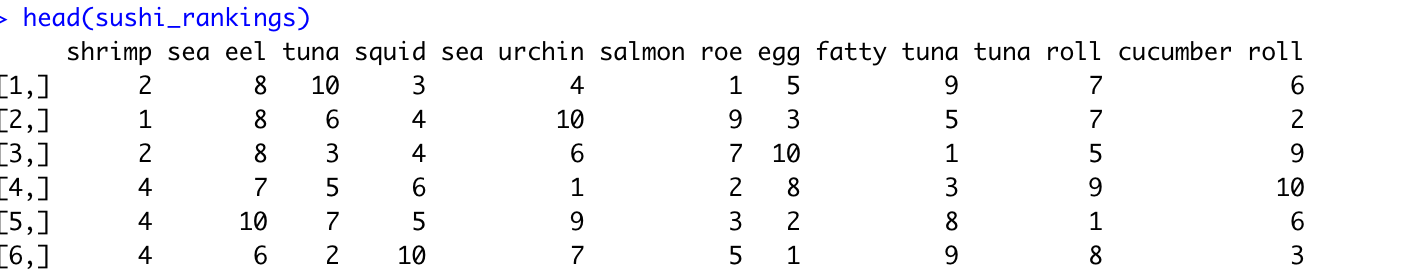
\includegraphics[width=10cm]{sushidata.png}
        \centering
    \end{figure}
\end{frame}

\begin{frame}{What we want to do?}
    \begin{itemize}
        \item Find consensus ranking of the items
        \item Extensions of model for pairwise comparisons, preference prediction and clustering.
    \end{itemize}
\end{frame}

\section{A Bayesian Mallows model for complete rankings}
\begin{frame}{Elementary settings}
\begin{itemize}
    \item Setting : $n$ items and $N$ assessors. $\mathbf{R}_j\in \mathcal{P}_n$ denotes the ranking(the full set of ranks given to the $n$ items) of assessor $j$ for each $j=1,\cdots, N$. ($\mathcal{P}_n$ is a permutation set)
    \item $d(\cdot\;,\; \cdot): \mathcal{P}_n\times \mathcal{P}_n\rightarrow [0,\infty)$ is a distance function between two rankings.
    \begin{itemize}
        \item Kendall distance : number of pairs of distinct elements whose order in the two rankings are the opposite.
        \item Footrule distance : $\ell_1$ distance
        \item Spearman's distance : $\ell_2$ distance 
    \end{itemize}
\end{itemize} 
\end{frame}

\begin{frame}{Mallows model}
\begin{itemize}
    \item Mallows model is a class of non-uniform joint distributions for a ranking $\mathbf{r}$ on $\mathcal{P}_n$. $$P(\mathbf{r}|\alpha, \boldsymbol{\rho})=Z_n(\alpha, \boldsymbol{\rho})^{-1}\exp\{-\frac{\alpha}{n}d(\mathbf{r}, \boldsymbol{\rho})\}I(\mathbf{r}\in \mathcal{P}_n) $$
    \item $\boldsymbol{\rho}\in \mathcal{P}_n$ is the latent consensus ranking. 
    \item $\alpha>0$ is a scale (or precision) parameter. \\i.e. $\alpha$ represents the level of agreement between assesssors, so that as $\alpha$ gets larger, ranking $\mathbf{r}$ aggregates more to $\boldsymbol{\rho}$ 
    \item $Z_n(\alpha, \boldsymbol{\rho})=\sum_{\mathbf{r}\in \mathcal{P}_n}e^{-\frac{\alpha}{n}d(\mathbf{r},\boldsymbol{\rho})}$ is the partition function.
    \begin{itemize}
        \item In physics, a `partition function' describes the statistical properties of a system in thermodynamic equilibrium. (Source : Wikipedia)
        \item Here, just consider this as a normalizing factor.
    \end{itemize}
\end{itemize} 
\end{frame}


\begin{frame}{Likelihood function}
\begin{itemize}
    \item Assume that observed rankings $\mathbf{R}_1, \cdots, \mathbf{R}_N$ are conditionally independent given $\alpha$ and $\boldsymbol{\rho}$ and each of them is distributed according to the Mallows model with these parameters.
    \item Likelihood takes the form as \begin{equation*}P(\mathbf{R}_1, \cdots, \mathbf{R}_N|\alpha, \boldsymbol{\rho})= Z_n(\alpha, \boldsymbol{\rho})^{-N}\exp\{-\frac{\alpha}{n}\sum_{j=1}^N d(\mathbf{R}_j, \boldsymbol{\rho})\}\prod_{j=1}^N I(\mathbf{R}_j\in \mathcal{P}_n) \end{equation*}
    \item For large $n$, finding the MLE of $\boldsymbol{\rho}$ given fixed $\alpha$ is not feasible because the space of permutations $\mathcal{P}_n$ has $n!$ elements. 
\end{itemize} 
\end{frame}

\begin{frame}{Right-invariant distance and partition function}
\begin{itemize}
    \item For any right-invariant distance, it holds $d(\mathbf{r}_1, \mathbf{r}_2)=d(\mathbf{r}_1 \mathbf{r}_2^{-1}, \mathbf{1}_n)$ where $\mathbf{1}_n=\{1,2,\cdots,n\}$ and $\mathbf{r}_1 \mapsto \mathbf{r}_1 \mathbf{r}_2^{-1}$ is relabelling map. Note that a right-invariant distance is unaffected by a relabelling of the items.
    \item Partition function $Z_n(\alpha, \boldsymbol{\rho})$ does not depend on $\boldsymbol{{\rho}}$. 
    \begin{align*}
    \because Z_n(\alpha, \boldsymbol{\rho}) &= \sum_{\mathbf{r}\in \mathcal{P}_n}\exp\{-\frac{\alpha}{n}d(\mathbf{r},\boldsymbol{\rho})\} = \sum_{\mathbf{r}\in \mathcal{P}_n}\exp\{-\frac{\alpha}{n}d(\mathbf{r} \boldsymbol{\rho}^{-1}, \mathbf{1}_n)\} \\ &=\sum_{\mathbf{r'}\in \mathcal{P}_n}\exp\{-\frac{\alpha}{n}d(\mathbf{r'},\mathbf{1}_n)\} \\ Z_n(\alpha, \boldsymbol{\rho}) &= Z_n(\alpha)=\sum_{\mathbf{r}\in \mathcal{P}_n}\exp\{-\frac{\alpha}{n}d(\mathbf{r},\mathbf{1}_n)\}
    \end{align*}
\end{itemize}
\end{frame}

\begin{frame}{Right-invariant distance and partition function}
\begin{itemize}
    \item For some choice of right-invariant distance like Kendall distance, the partition function can be analytically computed. 
    \item But there are important and natural right-invariant distances for which the computation of the partition function is not feasible, such as the footrule distance and the Spearman's distance.
\end{itemize}
\end{frame}

\begin{frame}{Prior distributions}
    \begin{itemize}
        \item Assume a priori that $\alpha$ and $\boldsymbol{\rho}$ are independent
        \item In this paper, the uniform prior $\pi(\boldsymbol{\rho})=\frac{1}{n!}I(\boldsymbol{\rho}\in \mathcal{P}_n)$ is employed.
        \item Also, for the scale parameter, this paper used a truncated exponential prior with density $\pi(\alpha | \lambda)=\lambda e^{-\lambda \alpha}I(\alpha\in [0, \alpha_{max}])/(1-e^{-\lambda \alpha_{max}})$ where the cut-off point $\alpha_{max}<\infty$ is large compared to the values supported by the data. In practice, in the computations involving the sampling of values for $\alpha$, truncation was never applied. We assign $\lambda$ a fixed value close to zero, implying a prior density for $\alpha$ which is quite flat.
        \begin{itemize}
            \item In short, prior $\alpha \sim Exp(\frac{1}{\lambda})$ with small $\lambda$ is used practically for $\alpha$. 
        \end{itemize}
    \end{itemize}
\end{frame}

\begin{frame}{Posterior distributions}
\begin{itemize}
    \item The posterior distribution for $\boldsymbol{\rho}$ and $\alpha$ is given by
    \begin{equation}
        P(\boldsymbol{\rho}, \alpha| \mathbf{R}_1, \cdots, \mathbf{R}_N)\propto \frac{\pi(\boldsymbol{\rho})\pi(\alpha)}{Z_n(\alpha)^N} \exp \big\{-\frac{\alpha}{n}\sum_{j=1}^N d(\mathbf{R}_j, \boldsymbol{\rho})\big\}
    \end{equation}
    \item The purpose of MCMC algorithm following is to obtain samples from this posterior.
\end{itemize}
\end{frame}

\begin{frame}{Metropolis-Hastings algorithm}
\begin{itemize}
    \item A general form of the Metropolis Hastings algorithm is as follows : \\ Target probability distribution is $p_0(x)$ for r.v. $X$. Given a current value $x^{(s)}$ of $X$, 
        \begin{enumerate}
            \item Generate $x^{*}$ from a proposal distribution $J_s(x^{*}|x^{(s)})$
            \item Compute the acceptance ratio $$ r=\frac{p_0(x^*)}{p_0(x^{(s)})}\, /\, \frac{J_s(x^*|x^{(s)})}{J_s(x^{(s)}|x^*)} = \frac{p_0(x^*)}{p_0(x^{(s)})}\frac{J_s(x^{(s)}|x^*)}{J_s(x^*|x^{(s)})} $$
            \item set $x^{(s+1)}$ to $x^*$ with probability $\min (1, r)$ \\ i.e. Sample $u\sim unif(0,1)$ and then if $u<r$ set $x^{(s+1)}=x^*$, else set $x^{(s+1)}=x^{(s)}$
        \end{enumerate}
    \item The primary restriction placed on $J_s(x^*|x^{(s)})$ is that it does not depend on values in the sequence previous to $x^{(s)}$ so that the algorithm generates a Markov chain.
    \item By Ergodic Thm, the empirical distribution of samples generated from such a Markov chain will converge to the stationary distribution( of the Markov chain), which agrees with the target distribution.
    \item Source : Hoff 2009. (textbook)
\end{itemize}
\end{frame}

\begin{frame}{Metropolis-Hastings Algorithm for Complete Rankings}
\begin{itemize}
    \item To obtain samples from the posterior distribution (1), we alternate between two steps.
    \begin{enumerate}
        \item Given $\alpha$ and $\boldsymbol{\rho}$, update $\boldsymbol{\rho}$ by proposing $\boldsymbol{\rho}'$
        \item Then, given $\alpha$ and $\boldsymbol{\rho}'$, update $\alpha$ by proposing $\alpha'$
    \end{enumerate}
\end{itemize}
\end{frame}

\begin{frame}{Updating $\boldsymbol{\rho}$}
\begin{itemize}
    \item Leap-and-Shift Proposal(L\&S)
    \item Leap step
        \begin{enumerate}
            \item Fix an integer $L\in \{1,2,\cdots, \floor{\frac{n-1}{2}}\}$ \\
            (which is a tuning parameter for MCMC algorithm)
            \item Draw a random number $u\sim Unif\{1,2,\cdots, n\}$
            \item Define $\mathcal{S}\subset \{1,2,\cdots, n\}$ by $\mathcal{S}=\big[\max (1, \rho_u-L), \min (n, \rho_u+L)\big]\diff\{\rho_u\}$
            \item Draw a random number $r\sim Unif(\mathcal{S})$
            \item Let $\boldsymbol{\rho}^*\in \{1,2,\cdots, n\}^n$ have elements $\begin{cases}
            \rho_i^*=\rho_i & i\in \{1,2,\cdots,n\}\diff \{u\} \\\rho_u^*=r \end{cases}$
             
        \end{enumerate}
\end{itemize}
\end{frame}

\begin{frame}{Updating $\boldsymbol{\rho}$}
\begin{itemize}
    \item Shift step
    \begin{enumerate}
        \item Let $\Delta=\rho_u^*-\rho_u$. Note that $\Delta\neq 0$ 
        \item Define the proposed $\boldsymbol{\rho}'\in \mathcal{P}_n$ by below :
        \begin{enumerate}
            \item If $\Delta>0$ then 
            $$\begin{cases}
                \rho_u'=\rho_u^* \\ \rho_i'=\rho_i-1 & if \; \rho_u<\rho_i\leq \rho_u^* \\ \rho_i'=\rho_i & otherwise
            \end{cases} $$
            \item If $\Delta<0$ then 
            $$\begin{cases}
                \rho_u'=\rho_u^* \\ \rho_i'=\rho_i+1 & if \; \rho_u>\rho_i\geq \rho_u^* \\ \rho_i'=\rho_i & otherwise
            \end{cases} $$
        \end{enumerate} 
    \end{enumerate}
\end{itemize}
\end{frame}

\begin{frame}{Updating $\boldsymbol{\rho}$}
\begin{itemize}
    \item Example of Leap and Shift proposal
    \begin{figure}
        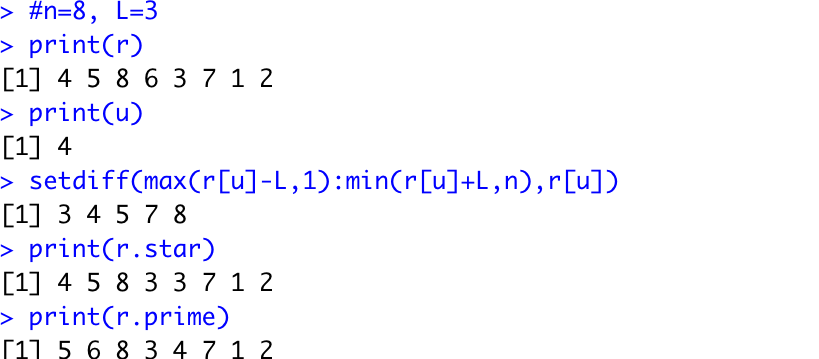
\includegraphics{LeapAndShift.png}
    \end{figure}
\end{itemize}
\end{frame}

\begin{frame}{Updating $\boldsymbol{\rho}$}
\begin{itemize}
    \item The probability mass function associated to the transition
    \begin{figure}
        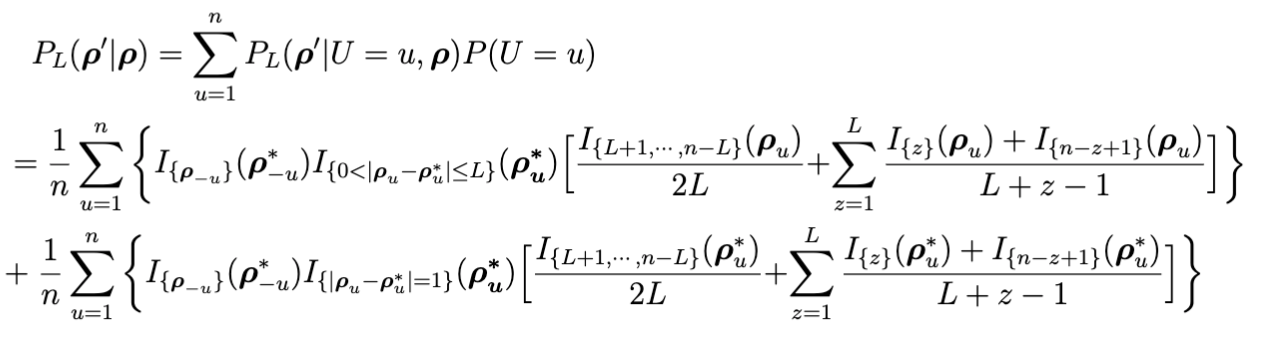
\includegraphics[width=11cm]{transitionProb.png}
    \end{figure}
\end{itemize}
\end{frame}

\begin{frame}{Updating $\boldsymbol{\rho}$}
\begin{itemize}
    \item Simple representation for the transition probability
        \begin{itemize}
            \item As we calculate $P(\boldsymbol{\rho}'|\boldsymbol{\rho})$, we should consider two random draws
            \begin{itemize}
                \item Draw $u\sim Unif\{1,2,\cdots, n\}$
                \item For $S$ dependent on $\boldsymbol{\rho}_u$, draw $r\sim Unif(S)$
                \item The other works including shift step involve no randomness.
            \end{itemize}
            \item Simply put, $P(\boldsymbol{\rho}'|\boldsymbol{\rho})=\frac{1}{n}\cdot\frac{1}{|S|}$ for many cases.
            \item However, if $|\boldsymbol{\rho}_u'-\boldsymbol{\rho}_u|=1$ then we should consider something more. 
            \item When $|\boldsymbol{\rho}_u'-\boldsymbol{\rho}_u|>1$ then $u$ is the only possible index that proposes $\boldsymbol{\rho}'$ from $\boldsymbol{\rho}$. On the other hand, when $|\boldsymbol{\rho}_u'-\boldsymbol{\rho}_u|=1$, there must be only one index $u'$ other than $u$ s.t. $|\boldsymbol{\rho}_{u'}'-\boldsymbol{\rho}_{u'}|=1$ so that $u'$ can also proposes $\boldsymbol{\rho}'$ from $\boldsymbol{\rho}$.
            \item In this special case, $P(\boldsymbol{\rho}'|\boldsymbol{\rho})=\frac{1}{n}\cdot\frac{1}{|S|}+\frac{1}{n}\cdot\frac{1}{|S'|}$ where $S$ is produced from drawing $u$ and $S'$ is produced from drawing $u'$
        \end{itemize}
\end{itemize}
\end{frame}

\begin{frame}{Updating $\boldsymbol{\rho}$}
\begin{itemize}
    \item example of leap and shift proposal  when $|\boldsymbol{\rho}_u'-\boldsymbol{\rho}_u|=1$
    \begin{figure}
        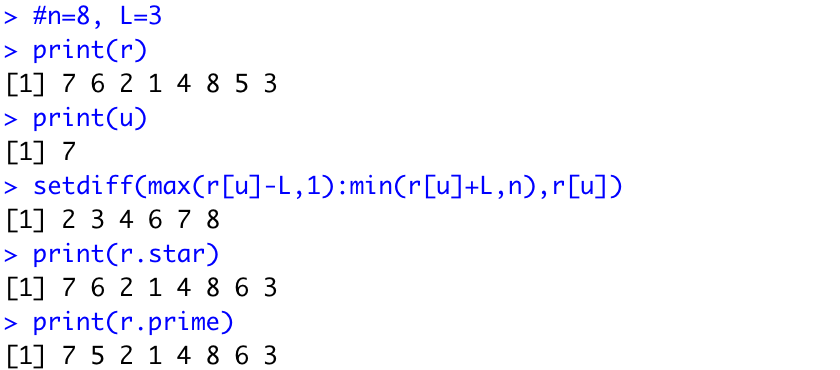
\includegraphics{LSproposal1.png}
    \end{figure}
\end{itemize}
\end{frame}

\begin{frame}{Updating $\boldsymbol{\rho}$}
\begin{itemize}
    \item Using this logic, we can rewrite the equality about $P_L(\boldsymbol{\rho}'|\boldsymbol{\rho})$ as the following 
    \begin{align*}
        P_L(\boldsymbol{\rho}'|\boldsymbol{\rho}) &= \sum_{u=1}^n P_L(\boldsymbol{\rho}'|U=u, \boldsymbol{\rho})P(U=u) \\ &= \frac{1}{n}\sum_{u=1}^n I(\boldsymbol{\rho}', \boldsymbol{\rho}, u) \frac{1}{|S^{(u)}|}
    \end{align*}
    where $I(\boldsymbol{\rho}', \boldsymbol{\rho}, u)$ is an indicator for possibility of proposal from $\boldsymbol{\rho}$ to $\boldsymbol{\rho}'$ given $u$ is drawed and $S^{(u)}$ is the set $S$ given $u$ is drawed \\ If $\boldsymbol{\rho}'$ is proposed from $\boldsymbol{\rho}$ then typically $I(\boldsymbol{\rho}', \boldsymbol{\rho}, u)=1$ for only one $u$ but if $|\boldsymbol{\rho}_u'-\boldsymbol{\rho}_u|=1$ then $I(\boldsymbol{\rho}', \boldsymbol{\rho}, u')=1$ also holds for another $u'$ different from $u$
\end{itemize}
\end{frame}

\begin{frame}{Updating $\boldsymbol{\rho}$}
\begin{itemize}
    \item The acceptance probability when updating $\boldsymbol{\rho}$ is 
        $\min\{1, r\}$ where $r$ is given as 
        \begin{align*}
            r &=\frac{P(\boldsymbol{\rho}', \alpha | \mathbf{R})}{P(\boldsymbol{\rho}, \alpha | \mathbf{R})}\cdot \frac{P_L(\boldsymbol{\rho}|\boldsymbol{\rho}')}{P_L(\boldsymbol{\rho}'|\boldsymbol{\rho})} \\ &= \frac{P_L(\boldsymbol{\rho}|\boldsymbol{\rho}')}{P_L(\boldsymbol{\rho}'|\boldsymbol{\rho})} \cdot \frac{\pi(\boldsymbol{\rho}')}{\pi(\boldsymbol{\rho})}\exp\big\{-\frac{\alpha}{n}\sum_{j=1}^N \big[d(\mathbf{R}_j, \boldsymbol{\rho}')-d(\mathbf{R}_j, \boldsymbol{\rho})\big] \big\}
        \end{align*} 
    \item Leap and shift proposal is not a symmetric proposal distribution. 
    \item The term $\sum_{j=1}^N \big[d(\mathbf{R}_j, \boldsymbol{\rho}')-d(\mathbf{R}_j, \boldsymbol{\rho})\big]$ above can be computed efficiently since most elements of $\boldsymbol{\rho}$ and $\boldsymbol{\rho}'$ are equal and we can put aside indices $i$ s.t. $\rho_i=\rho'_i$
\end{itemize}
\end{frame}

\begin{frame}{Metropolis-Hastings Algorithm for Complete Rankings}
\begin{itemize}
    \item To obtain samples from the posterior distribution (1), we alternate between two steps.
    \begin{enumerate}
        \item Given $\alpha$ and $\boldsymbol{\rho}$, update $\boldsymbol{\rho}$ by proposing $\boldsymbol{\rho}'$
        \item Then, given $\alpha$ and $\boldsymbol{\rho}'$, update $\alpha$ by proposing $\alpha'$
    \end{enumerate}
\end{itemize}
\end{frame}

\begin{frame}{Metropolis-Hastings Algorithm for Complete Rankings}
\begin{itemize}
    \item To obtain samples from the posterior distribution (1), we alternate between two steps.
    \begin{enumerate}
        \item Given $\alpha$ and $\boldsymbol{\rho}$, update $\boldsymbol{\rho}$ by proposing $\boldsymbol{\rho}'$
        \item Then, given $\alpha$ and $\boldsymbol{\rho}'$, update $\alpha$ by proposing $\alpha'$
    \end{enumerate}
\end{itemize}
\end{frame}

\begin{frame}{Metropolis-Hastings Algorithm for Complete Rankings}
\begin{itemize}
    \item To obtain samples from the posterior distribution (1), we alternate between two steps.
    \begin{enumerate}
        \item Given $\alpha$ and $\boldsymbol{\rho}$, update $\boldsymbol{\rho}$ by proposing $\boldsymbol{\rho}'$
        \item Then, given $\alpha$ and $\boldsymbol{\rho}'$, update $\alpha$ by proposing $\alpha'$
    \end{enumerate}
\end{itemize}
\end{frame}

\begin{frame}{Metropolis-Hastings Algorithm for Complete Rankings}
\begin{itemize}
    \item To obtain samples from the posterior distribution (1), we alternate between two steps.
    \begin{enumerate}
        \item Given $\alpha$ and $\boldsymbol{\rho}$, update $\boldsymbol{\rho}$ by proposing $\boldsymbol{\rho}'$
        \item Then, given $\alpha$ and $\boldsymbol{\rho}'$, update $\alpha$ by proposing $\alpha'$
    \end{enumerate}
\end{itemize}
\end{frame}

\begin{frame}{Metropolis-Hastings Algorithm for Complete Rankings}
\begin{itemize}
    \item To obtain samples from the posterior distribution (1), we alternate between two steps.
    \begin{enumerate}
        \item Given $\alpha$ and $\boldsymbol{\rho}$, update $\boldsymbol{\rho}$ by proposing $\boldsymbol{\rho}'$
        \item Then, given $\alpha$ and $\boldsymbol{\rho}'$, update $\alpha$ by proposing $\alpha'$
    \end{enumerate}
\end{itemize}
\end{frame}

\begin{frame}{Metropolis-Hastings Algorithm for Complete Rankings}
\begin{itemize}
    \item To obtain samples from the posterior distribution (1), we alternate between two steps.
    \begin{enumerate}
        \item Given $\alpha$ and $\boldsymbol{\rho}$, update $\boldsymbol{\rho}$ by proposing $\boldsymbol{\rho}'$
        \item Then, given $\alpha$ and $\boldsymbol{\rho}'$, update $\alpha$ by proposing $\alpha'$
    \end{enumerate}
\end{itemize}
\end{frame}

\begin{frame}{Metropolis-Hastings Algorithm for Complete Rankings}
\begin{itemize}
    \item To obtain samples from the posterior distribution (1), we alternate between two steps.
    \begin{enumerate}
        \item Given $\alpha$ and $\boldsymbol{\rho}$, update $\boldsymbol{\rho}$ by proposing $\boldsymbol{\rho}'$
        \item Then, given $\alpha$ and $\boldsymbol{\rho}'$, update $\alpha$ by proposing $\alpha'$
    \end{enumerate}
\end{itemize}
\end{frame}

\begin{frame}{Metropolis-Hastings Algorithm for Complete Rankings}
\begin{itemize}
    \item To obtain samples from the posterior distribution (1), we alternate between two steps.
    \begin{enumerate}
        \item Given $\alpha$ and $\boldsymbol{\rho}$, update $\boldsymbol{\rho}$ by proposing $\boldsymbol{\rho}'$
        \item Then, given $\alpha$ and $\boldsymbol{\rho}'$, update $\alpha$ by proposing $\alpha'$
    \end{enumerate}
\end{itemize}
\end{frame}

\begin{frame}{Metropolis-Hastings Algorithm for Complete Rankings}
\begin{itemize}
    \item To obtain samples from the posterior distribution (1), we alternate between two steps.
    \begin{enumerate}
        \item Given $\alpha$ and $\boldsymbol{\rho}$, update $\boldsymbol{\rho}$ by proposing $\boldsymbol{\rho}'$
        \item Then, given $\alpha$ and $\boldsymbol{\rho}'$, update $\alpha$ by proposing $\alpha'$
    \end{enumerate}
\end{itemize}
\end{frame}

\begin{frame}{Metropolis-Hastings Algorithm for Complete Rankings}
\begin{itemize}
    \item To obtain samples from the posterior distribution (1), we alternate between two steps.
    \begin{enumerate}
        \item Given $\alpha$ and $\boldsymbol{\rho}$, update $\boldsymbol{\rho}$ by proposing $\boldsymbol{\rho}'$
        \item Then, given $\alpha$ and $\boldsymbol{\rho}'$, update $\alpha$ by proposing $\alpha'$
    \end{enumerate}
\end{itemize}
\end{frame}

\begin{frame}{Metropolis-Hastings Algorithm for Complete Rankings}
\begin{itemize}
    \item To obtain samples from the posterior distribution (1), we alternate between two steps.
    \begin{enumerate}
        \item Given $\alpha$ and $\boldsymbol{\rho}$, update $\boldsymbol{\rho}$ by proposing $\boldsymbol{\rho}'$
        \item Then, given $\alpha$ and $\boldsymbol{\rho}'$, update $\alpha$ by proposing $\alpha'$
    \end{enumerate}
\end{itemize}
\end{frame}

\begin{frame}{Metropolis-Hastings Algorithm for Complete Rankings}
\begin{itemize}
    \item To obtain samples from the posterior distribution (1), we alternate between two steps.
    \begin{enumerate}
        \item Given $\alpha$ and $\boldsymbol{\rho}$, update $\boldsymbol{\rho}$ by proposing $\boldsymbol{\rho}'$
        \item Then, given $\alpha$ and $\boldsymbol{\rho}'$, update $\alpha$ by proposing $\alpha'$
    \end{enumerate}
\end{itemize}
\end{frame}

\begin{frame}{Metropolis-Hastings Algorithm for Complete Rankings}
\begin{itemize}
    \item To obtain samples from the posterior distribution (1), we alternate between two steps.
    \begin{enumerate}
        \item Given $\alpha$ and $\boldsymbol{\rho}$, update $\boldsymbol{\rho}$ by proposing $\boldsymbol{\rho}'$
        \item Then, given $\alpha$ and $\boldsymbol{\rho}'$, update $\alpha$ by proposing $\alpha'$
    \end{enumerate}
\end{itemize}
\end{frame}

\begin{frame}{Metropolis-Hastings Algorithm for Complete Rankings}
\begin{itemize}
    \item To obtain samples from the posterior distribution (1), we alternate between two steps.
    \begin{enumerate}
        \item Given $\alpha$ and $\boldsymbol{\rho}$, update $\boldsymbol{\rho}$ by proposing $\boldsymbol{\rho}'$
        \item Then, given $\alpha$ and $\boldsymbol{\rho}'$, update $\alpha$ by proposing $\alpha'$
    \end{enumerate}
\end{itemize}
\end{frame}

\begin{frame}{Metropolis-Hastings Algorithm for Complete Rankings}
\begin{itemize}
    \item To obtain samples from the posterior distribution (1), we alternate between two steps.
    \begin{enumerate}
        \item Given $\alpha$ and $\boldsymbol{\rho}$, update $\boldsymbol{\rho}$ by proposing $\boldsymbol{\rho}'$
        \item Then, given $\alpha$ and $\boldsymbol{\rho}'$, update $\alpha$ by proposing $\alpha'$
    \end{enumerate}
\end{itemize}
\end{frame}

\begin{frame}{Metropolis-Hastings Algorithm for Complete Rankings}
\begin{itemize}
    \item To obtain samples from the posterior distribution (1), we alternate between two steps.
    \begin{enumerate}
        \item Given $\alpha$ and $\boldsymbol{\rho}$, update $\boldsymbol{\rho}$ by proposing $\boldsymbol{\rho}'$
        \item Then, given $\alpha$ and $\boldsymbol{\rho}'$, update $\alpha$ by proposing $\alpha'$
    \end{enumerate}
\end{itemize}
\end{frame}

\begin{frame}{Metropolis-Hastings Algorithm for Complete Rankings}
\begin{itemize}
    \item To obtain samples from the posterior distribution (1), we alternate between two steps.
    \begin{enumerate}
        \item Given $\alpha$ and $\boldsymbol{\rho}$, update $\boldsymbol{\rho}$ by proposing $\boldsymbol{\rho}'$
        \item Then, given $\alpha$ and $\boldsymbol{\rho}'$, update $\alpha$ by proposing $\alpha'$
    \end{enumerate}
\end{itemize}
\end{frame}

\begin{frame}{Metropolis-Hastings Algorithm for Complete Rankings}
\begin{itemize}
    \item To obtain samples from the posterior distribution (1), we alternate between two steps.
    \begin{enumerate}
        \item Given $\alpha$ and $\boldsymbol{\rho}$, update $\boldsymbol{\rho}$ by proposing $\boldsymbol{\rho}'$
        \item Then, given $\alpha$ and $\boldsymbol{\rho}'$, update $\alpha$ by proposing $\alpha'$
    \end{enumerate}
\end{itemize}
\end{frame}

\begin{frame}{Metropolis-Hastings Algorithm for Complete Rankings}
\begin{itemize}
    \item To obtain samples from the posterior distribution (1), we alternate between two steps.
    \begin{enumerate}
        \item Given $\alpha$ and $\boldsymbol{\rho}$, update $\boldsymbol{\rho}$ by proposing $\boldsymbol{\rho}'$
        \item Then, given $\alpha$ and $\boldsymbol{\rho}'$, update $\alpha$ by proposing $\alpha'$
    \end{enumerate}
\end{itemize}
\end{frame}

\begin{frame}{Metropolis-Hastings Algorithm for Complete Rankings}
\begin{itemize}
    \item To obtain samples from the posterior distribution (1), we alternate between two steps.
    \begin{enumerate}
        \item Given $\alpha$ and $\boldsymbol{\rho}$, update $\boldsymbol{\rho}$ by proposing $\boldsymbol{\rho}'$
        \item Then, given $\alpha$ and $\boldsymbol{\rho}'$, update $\alpha$ by proposing $\alpha'$
    \end{enumerate}
\end{itemize}
\end{frame}

\begin{frame}{Metropolis-Hastings Algorithm for Complete Rankings}
\begin{itemize}
    \item To obtain samples from the posterior distribution (1), we alternate between two steps.
    \begin{enumerate}
        \item Given $\alpha$ and $\boldsymbol{\rho}$, update $\boldsymbol{\rho}$ by proposing $\boldsymbol{\rho}'$
        \item Then, given $\alpha$ and $\boldsymbol{\rho}'$, update $\alpha$ by proposing $\alpha'$
    \end{enumerate}
\end{itemize}
\end{frame}

\begin{frame}{Metropolis-Hastings Algorithm for Complete Rankings}
\begin{itemize}
    \item To obtain samples from the posterior distribution (1), we alternate between two steps.
    \begin{enumerate}
        \item Given $\alpha$ and $\boldsymbol{\rho}$, update $\boldsymbol{\rho}$ by proposing $\boldsymbol{\rho}'$
        \item Then, given $\alpha$ and $\boldsymbol{\rho}'$, update $\alpha$ by proposing $\alpha'$
    \end{enumerate}
\end{itemize}
\end{frame}

\begin{frame}{Metropolis-Hastings Algorithm for Complete Rankings}
\begin{itemize}
    \item To obtain samples from the posterior distribution (1), we alternate between two steps.
    \begin{enumerate}
        \item Given $\alpha$ and $\boldsymbol{\rho}$, update $\boldsymbol{\rho}$ by proposing $\boldsymbol{\rho}'$
        \item Then, given $\alpha$ and $\boldsymbol{\rho}'$, update $\alpha$ by proposing $\alpha'$
    \end{enumerate}
\end{itemize}
\end{frame}

\begin{frame}{Metropolis-Hastings Algorithm for Complete Rankings}
\begin{itemize}
    \item To obtain samples from the posterior distribution (1), we alternate between two steps.
    \begin{enumerate}
        \item Given $\alpha$ and $\boldsymbol{\rho}$, update $\boldsymbol{\rho}$ by proposing $\boldsymbol{\rho}'$
        \item Then, given $\alpha$ and $\boldsymbol{\rho}'$, update $\alpha$ by proposing $\alpha'$
    \end{enumerate}
\end{itemize}
\end{frame}


%\subsection<presentation>*{For Further Reading}
\begin{frame}[t, allowframebreaks]
\frametitle{References}
\bibliographystyle{dcu}
\bibliography{c}
\end{frame}


\end{document}
